% Rule sheet for primes game
% Game design: Grant Sinclair
% Graphic design: Harald Bögeholz

\documentclass{article}

\usepackage[a4paper, left=5cm, right=5cm, top=3cm, bottom=3cm]{geometry}

\usepackage{fontspec}
\usepackage{graphicx}
\usepackage{adjustbox}

% For custom header and footer
\usepackage{fancyhdr}

% For custom date format
\usepackage[useregional=numeric]{datetime2}

\pagestyle{fancy}
\fancyhf{} % clear all header and footer fields
\renewcommand{\headrulewidth}{0pt} % no line in header area
\fancyfoot[L]{Skip or Trip} % left footer
\fancyfoot[C]{\thepage} % center footer
\fancyfoot[R]{\DTMtoday} % right footer

\setmainfont{HelveticaNeue}

\newcommand{\card}[1]{\adjustbox{valign=m}{\includegraphics[page=#1, width=2cm]{primecards-screen.pdf}}}
\newcommand{\largecard}[1]{\adjustbox{valign=m}{\includegraphics[page=#1, width=45mm]{primecards-screen.pdf}}}
\newcommand{\square}[1]{\adjustbox{valign=m}{
\includegraphics[page=#1, width=2cm]{boardsquares.pdf}}}

\setlength{\parindent}{0pt}

\begin{document}

{\center\LARGE\textbf{Skip or Trip -- a game for 2 to 6 players}}

\section*{Setup}

Each player starts with a single token on the starting square. Shuffle the deck. If there are exactly five players, discard  eight cards. Deal two cards to each player and place the deck black side up. Players should hold their cards so only they can see the symbols on the white sides of their cards, but the numbers on the black sides are visible to their opponents.

\section*{Gameplay}

Players take turns in a clockwise direction. On their turn, a player either \textbf{skips} or \textbf{trips}.

\begin{description}

\item[Skip:] Play a single card with the black side up and skip forward by the number on the card.

\item[Trip:] Play any number of cards with the white side up such that the symbols on the cards \textit{exactly match} the symbols on a square occupied by an opponent. Move the opponent's token back by the sum of the numbers on the cards and \textit{then} move your own token forward by the same number. After tripping an opponent, the player may trip again as many times as they can and want, but they may not skip any more on this turn.

\end{description}

Each square can only have one token on it. If a token is moved to an occupied square, the other token gets pushed back one square. If that square is occupied, its token gets pushed back by one and so forth. The only square that can have multiple tokens on it is the starting square. A token cannot be tripped below zero and will stop at the starting square rather than be tripped further back. Square 100 has to be reached exactly; if a token is too close to 100 and the number to move is too large, the token has to stay in place. 

At the end of their turn, the player \textbf{draws two cards} and puts all cards they played into the discard pile. Discarded cards are not reused; when the deck runs out, the players stop drawing and the endgame starts.
 
\section*{End of the game}

When a player gets to 100, they win the game. If the deck runs out before that, the \textbf{endgame} starts: If a player is in the last position at the end of their turn, they quit the game and remove their token. The winner is the player who remains at the end.

\section*{Example}

Let's say on Yellow's turn Blue's token is on square \square{12} and Red's token is on square~\square{5}.

Yellow trips by playing \card{91} \card{69} for a total of 7, taking Blue from \square{12} back to \square{5} and pushing Red from \square{5} back to~\square{4}. Yellow moves forward 7 squares.

Yellow now trips again by playing \card{125}, sending Blue back from \square{5} to the starting square. They move their own token forward 6 squares and end their turn, discarding all cards from play and drawing two cards.

It is now Red's turn. Red plays~\card{170} and moves their token forward 8 squares, landing on~\square{12}. They discard the card from play and draw two cards.


\section*{Optional rule for 4--6 players: Mercy}

The token in the last position cannot be tripped.

\section*{Advanced Rules for 2--3 players}

Rules are the same as above unless noted. Each player has two tokens of the same colour.
The deck is cut after shuffling. The Mercy rule does not apply. 
The \textbf{winner} is the player whose \textbf{last token is furthest ahead} when the game ends. 
Players cannot move a token to 100 unless doing so wins them the game.

\section*{Team play for 4 players (2 teams of 2)}

Rules are the same as the Advanced Rules unless noted.
Players sit opposite their partner. 
Partners are not allowed to discuss strategy with each other.
Each pair of players has two tokens of the same colour.

\newpage
\section*{About the cards}

The deck has 108 cards, 12 for each number from 1 to~9. For each number, the back (black side) of the card shows which 12 symbols (or combinations of symbols) are on the white side of cards with that number.

\begin{adjustbox}{center}
\begin{tabular}{ccc}
\vspace*{5pt}\\
\largecard{2} & \largecard{26} & \largecard{50} \vspace*{10pt}\\
\largecard{74} & \largecard{98} & \largecard{122} \vspace*{10pt}\\
\largecard{146} & \largecard{170} & \largecard{194} \vspace*{10pt}\\
\end{tabular}
\end{adjustbox}

\end{document}
